\section{Intuition for the polarization structure of magnetized filaments}
\begin{figure}
  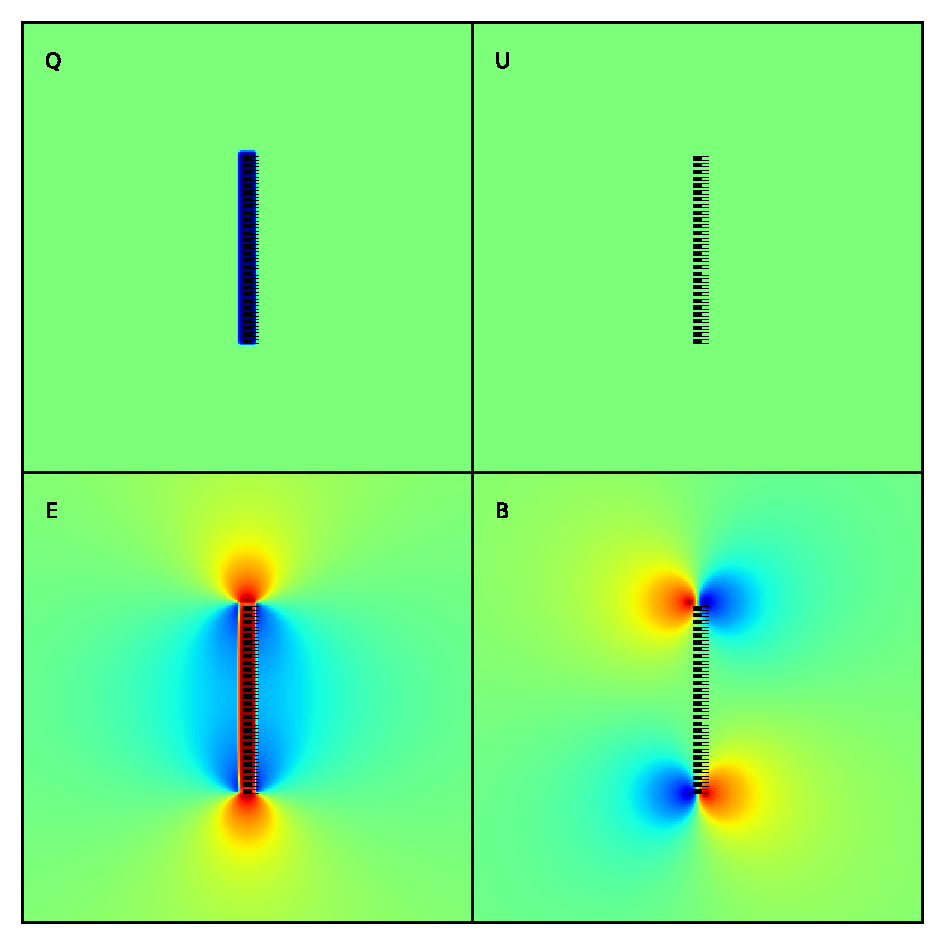
\includegraphics[width=0.5\columnwidth]{line.pdf}
  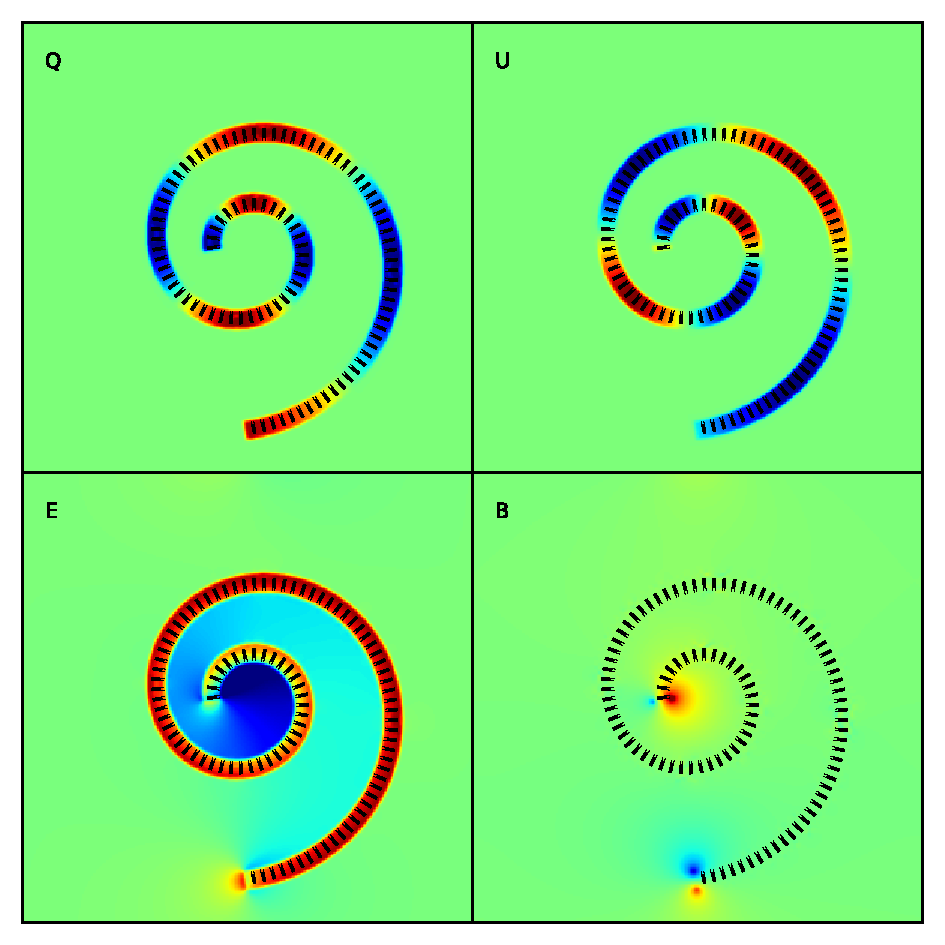
\includegraphics[width=0.5\columnwidth]{spiral.pdf}
  \caption{
    The polarization signals of toy filament structures.
    In a filament organized perfectly along a magnetic field line, the polarization will be perpendicular to the filament direction.  The $E/B$ modes of filaments are in some ways easier to think about than the Stokes parameters.
    Left panels: in a straight filament, the E-mode is positive along the filament and at the ends, but negative along the sides.  B-modes are only non-zero at the ends.  Right panels: in a curved filament, the E-mode is again positive along the filament.  Outside the filament, the $E$-mode is more negative on the interior of the curve than the exterior.  The $B$-modes are again non-zero only at the ends, and are akin to the straight filament case.
    In all images, the longitude increases to the left (sky convention).}
  \label{fig:polfilaments}
\end{figure}

Naturally describes the reason for a positive T/E correlation.  Figure~\ref{fig:polfilaments}.
